\subsection{Rekursionsschnecke}

\begin{figure}[H]
	\centering
    \includegraphics[scale=0.6]{grafiken/Rekursionsschnecke.eps}
	\caption{Die \enquote{Rekursionsschnecke}}\label{fig:rekusionsschnecke}
\end{figure}

\paragraph{Aufgabe 1}

\[
    a_n =\ ?
\]

\paragraph{Lösungsweg}

\subparagraph{Satz des Pythagoras}

\begin{align*}  
    a_1^2 + a_1^2 &= D^2 \\
    2 a_1^2 &= 10^2 \\
    a_1^2 &= 50 \\
    a_1 &= \sqrt{50}
\end{align*}

\begin{align*}
    a_2^2 + a_2^2 &= a_1^2 \\
    2 a_2^2 &= {\sqrt{50}}^2 \\
    a_2^2 &= \frac{50}{2} \\
    a_2 &= \sqrt{\frac{50}{2}} = \sqrt{50} \cdot \frac{1}{\sqrt{2}}
\end{align*}

\begin{align*}
    a_3^2 + a_3^2 &= a_2^2 \\
    2 a_3^2 &= \frac{50}{2} \\
    a_3^2 &= \frac{50}{4} \\
    a_3 &= \sqrt{50} \cdot \frac{1}{\sqrt{4}}
\end{align*}

\[
    \langle a_n \rangle = \sqrt{50},\ \sqrt{50} \cdot \frac{1}{\sqrt{2}},\ \sqrt{50} \cdot \frac{1}{\sqrt{4}},\ \ldots \
\]

\subparagraph{geometrische Folge}

\begin{align*}
    a_n &= a \cdot q^{n-1} \\
    a_n &= \sqrt{50} \cdot \sqrt{\frac{1}{2^{n-1}}} \\
    &= \sqrt{50} \cdot {\left(\frac{1}{\sqrt{2}}\right)}^{n-1} \\
    \Rightarrow q &= \frac{1}{\sqrt{2}}
\end{align*}

\paragraph{Aufgabe 2}

\[
    S =\ ?
\]

\paragraph{Lösungsweg}

\[
    S = a \cdot \frac{1 - q^n}{1 - q} = \sqrt{50} \cdot \frac{1}{1- \frac{1}{\sqrt{2}}} \approx 24,14
\]
